\section{Auswertung}
\label{sec:Auswertung}
\subsection{Überprüfung der Bragg Bedingung}
\label{sec:Überprüfung der Bragg Bedingung}
Aus der folgenden Graphik und den dazugehörigen Messwerten in Tabelle $\ref{table:A2}$ kann das Maximum der Kurve bei
\begin{align*}
  \theta = 13.8 \si{\degree}
\end{align*}
entnommen werden.
\begin{figure}
  \centering
  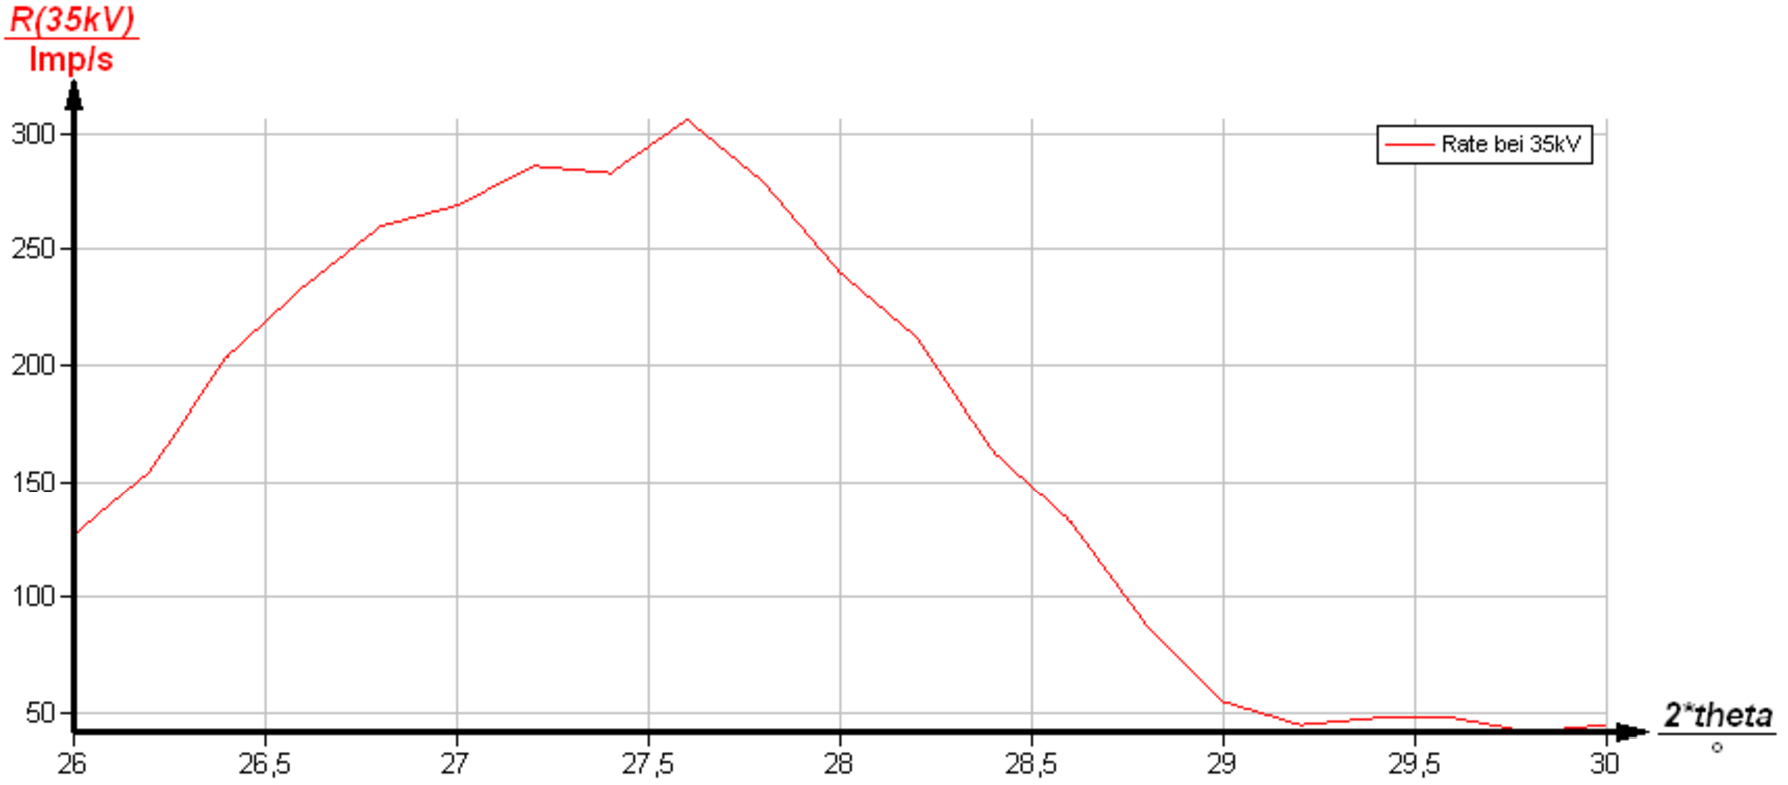
\includegraphics[width=\textwidth]{ressources/1.Messung.pdf}
  \caption{Überprüfung des Bragg Bedingung.}
  \label{fig:plot1}
\end{figure}

\input{build/Tabelle_messung_1_texformat.tex}
\newpage


\subsection{Das Emissionsspektrum einer Cu-Röntgenröhre}
\label{sec:Das Emissionsspektrum einer Cu-Röntgenröhre}
In Abbildung $\ref{fig:plot2}$ ist das Emissionsspektrum der Kupferanode mit den charakteristischen, lokalen Maxima dargestellt.
\begin{figure}[H]
  \centering
  \includegraphics[width=\textwidth]{build/cu-emission.pdf}
  \caption{Emissionsspektrum der Kupferanode.}
  \label{fig:plot2}
\end{figure}

\subsubsection{Grenzwinkel}
\label{sec:Grenzwinkel}
Anhand des Grenzwinkels, der nach Abbildung $\ref{fig:plot2}$ bei $\theta _\textrm{G} = 5.4 \si{\degree}$ liegt, wird mit Gleichung \ref{eq:bragg} die
minimale Wellenlänge $\lambda_\textrm{min}$ bzw. die maximale Energie $E_\textrm{max}$ des Bremsspektrums bestimmt.
\begin{align*}
  \lambda_\textrm{min} &= \input{build/lambda_min.tex} \\
  E_\textrm{max} &= \input{build/E_max.tex}
\end{align*}

\subsubsection{Halbwertsbreite}
\label{sec:Halbwertsbreite}
Für die Berechnung der Halbwertsbreite $\Delta \theta$ wird das Emissionsspektrum nur in der Umgebung um $K_\alpha$ und $K_\beta$ betrachtet. Die Spline-Interpolation dieser beiden Umgebungen sind in Abbildung $\ref{fig:plot3}$ und $\ref{fig:plot4}$  dargestellt.

\begin{figure}[H]
  \centering
  \includegraphics[width=\textwidth]{build/halbwertsbreiten_alpha.pdf}
  \caption{Interpolation der $K_\alpha$ - Umgebung.}
  \label{fig:plot3}
\end{figure}

\begin{figure}[H]
  \centering
  \includegraphics[width=\textwidth]{build/halbwertsbreiten_beta.pdf}
  \caption{Interpolation der $K_\beta$ - Umgebung.}
  \label{fig:plot4}
\end{figure}
Mit der Bragg'schen Bedingung und Gleichung \ref{eq:Ephoton} wird die Halbwertsbreite $\Delta \theta$ und das Auflösungsvermögen $\Delta E$ bestimmt.

\begin{align*}
  \Delta \theta_{\text{K}_\alpha} &= \input{build/Halbwertsbreite_alpha.tex}\\
  \Delta E_{\text{K}_\alpha} &= \input{build/Energieaufloesung_alpha.tex}\\
  \\
  \Delta \theta_{\text{K}_\beta} &= \input{build/Halbwertsbreite_beta.tex}\\
  \Delta E_{\text{K}_\beta} &= \input{build/Energieaufloesung_beta.tex}
\end{align*}

\subsubsection{Abschirmkonstante}
\label{sec:Abschirmkonstante}
Aus Abbildung $\ref{fig:plot2}$ werden die Winkel der $K_\alpha$- und $K_\beta$-Maxima bei
\begin{align*}
  \theta_{\text{K}_\alpha} &= \input{build/theta_alpha.tex}\\
  \theta_{\text{K}_\beta} &= \input{build/theta_beta.tex}
\end{align*}
abgelesen.
Mit der Bragg'schen Bedingung wird die dazugehörige Energie $E$ berechnet, weiter werden durch Umstellung bzw. Aufteilung von Gleichung \ref{eq:sigma_k}
\begin{align}
  \sigma_{\text{K}_\beta} &=  z_\textrm{Kupfer} - \sqrt{\frac{E_{\text{K}_\beta}}{R_\infty}}\\
  \sigma_{\text{K}_\alpha} &=  z_\textrm{Kupfer} -2\sqrt{\frac{R_\infty(z_\textrm{Kupfer} - \sigma_{\text{K}_\beta})^2 - E_{\text{K}_\alpha} }{R_\infty}}
\end{align}
die Abschirmkonstanten $\sigma_{\text{K}_\alpha} , \sigma_{\text{K}_\beta}$ ermittelt.
\begin{align*}
  \sigma_{\text{K}_\alpha} &= \input{build/sigma_1.tex}\\
  \sigma_{\text{K}_\beta} &= \input{build/sigma_2.tex}
\end{align*}
% \begin{align}
%   \Delta \theta_\beta &= \input{build/Energiedifferenz.tex}\\
% \end{align}
\subsection{Das Absorptionsspektrum verschiedener Absorber}
\label{sec:Das Absorptionsspektrum}
In den Abbildungen $\ref{fig:plot5}$ - $\ref{fig:plot8}$ sind die gemessenen Absorptionsspektren von Germanium, Gold, Zink und Zirkonium dargestellt.

\begin{figure}[H]
  \centering
  \includegraphics[width=\textwidth]{build/Germanium.pdf}
  \caption{Absorptionsspektrum von Germanium.}
  \label{fig:plot5}
\end{figure}

\begin{figure}[H]
  \centering
  \includegraphics[width=\textwidth]{build/Zink.pdf}
  \caption{Absorptionsspektrum von Zink.}
  \label{fig:plot6}
\end{figure}

\begin{figure}[H]
  \centering
  \includegraphics[width=\textwidth]{build/Zirkonium.pdf}
  \caption{Absorptionsspektrum von Zirkonium.}
  \label{fig:plot7}
\end{figure}

\begin{figure}[H]
  \centering
  \includegraphics[width=\textwidth]{build/Gold.pdf}
  \caption{Absorptionsspektrum Gold.}
  \label{fig:plot8}
\end{figure}

Durch eine lineare Näherung der jeweiligen Kantenübergänge ergeben sich die Absorptionswinkel $\theta_{\text{K}_\alpha}$, wodruch mit Gleichung \ref{eq:Ephoton}
die  Absorptionsenergien $E_{\text{K}_\alpha} $ berechnet werden. Die Ergebnisse sind in der folgenden Tabelle aufgelistet.

\begin{table}
  \centering
  \begin{tabular}{lS}
    \toprule
    & {$E_{\text{K}_\alpha} \:/\: \si{\kilo\electronvolt}$} \\
    \midrule
    Ge (Germanium)     & $\input{build/Absorptionsenergie_Germanium_ohne.tex} $  \\
    Zn (Zink)          & $\input{build/Absorptionsenergie_Zink_ohne.tex} $       \\
    Zr (Zirkonium)     & $\input{build/Absorptionsenergie_Zirkonium_ohne.tex} $   \\
    \bottomrule
  \end{tabular}
  \caption{Auflistung der Absorptionsenergien $E_{\text{K}_\alpha} $.}
  \label{tab:2}
\end{table}

Mit den zuvor berechneten Absorptionsenergien $E_{\text{K}_\alpha} $ werden gemäß
\begin{align}
  \sigma_{\text{K}_\alpha} = z - \sqrt{\frac{E_{\text{K}_\alpha}}{R_\infty}-\frac{\alpha}{4}z^4}
\end{align}
die jeweiligen Abschirmkonstanten der drei Absorber berechnet. Die Ergebnisse sind in der folgenden Tabelle zusammengefasst.

\begin{table}
  \centering
  \begin{tabular}{lS}
    \toprule
    & {$\sigma_{\text{K}_\alpha}$} \\
    \midrule
    Ge (Germanium)     & $\input{build/Abschirmkonstante_Germanium.tex} $  \\
    Zn (Zink)          & $\input{build/Abschirmkonstante_Zink.tex} $       \\
    Zr (Zirkonium)     & $\input{build/Abschirmkonstante_Zirkonium.tex} $   \\
    \bottomrule
  \end{tabular}
  \caption{Auflistung der Abschirmkonstanten $\sigma $.}
  \label{tab:3}
\end{table}



\subsection{Moseleysches Gesetz}
\label{sec:Moseleysches Gesetz}
In Abbildung $\ref{fig:plot9}$ ist die Wurzel aus den in Kapitel $\ref{sec:Das Absorptionsspektrum}$ berecheten Absorptionsenergien $ \sqrt{E_{\text{K}_\alpha}} $ gegen die Kernladungszahlen $Z$ aufgetragen. Aus der Steigung des linearen Zusammenhangs, lässt sich auf die Rydbergkonstante $R_\infty$ schließen.

\begin{align*}
  hc R_\infty &= \input{build/hcRydbergonstante.tex}\\
  R_\infty   &= \input{build/Rydbergonstante.tex}
\end{align*}

\begin{figure}[H]
  \centering
  \includegraphics[width=\textwidth]{build/Moseley_Diagramm.pdf}
  \caption{Moseley-Diagramm.}
  \label{fig:plot9}
\end{figure}


% % Examples
% \begin{equation}
%   U(t) = a \sin(b t + c) + d
% \end{equation}
%
% \begin{align}
%   a &= \input{build/a.tex} \\
%   b &= \input{build/b.tex} \\
%   c &= \input{build/c.tex} \\
%   d &= \input{build/d.tex} .
% \end{align}
% Die Messdaten und das Ergebnis des Fits sind in Abbildung~\ref{fig:plot} geplottet.
%
% %Tabelle mit Messdaten
% \begin{table}
%   \centering
%   \caption{Messdaten.}
%   \label{tab:data}
%   \sisetup{parse-numbers=false}
%   \begin{tabular}{
% % format 1.3 bedeutet eine Stelle vorm Komma, 3 danach
%     S[table-format=1.3]
%     S[table-format=-1.2]
%     @{${}\pm{}$}
%     S[table-format=1.2]
%     @{\hspace*{3em}\hspace*{\tabcolsep}}
%     S[table-format=1.3]
%     S[table-format=-1.2]
%     @{${}\pm{}$}
%     S[table-format=1.2]
%   }
%     \toprule
%     {$t \:/\: \si{\milli\second}$} & \multicolumn{2}{c}{$U \:/\: \si{\kilo\volt}$\hspace*{3em}} &
%     {$t \:/\: \si{\milli\second}$} & \multicolumn{2}{c}{$U \:/\: \si{\kilo\volt}$} \\
%     \midrule
%     1.7 & 10 \\
2.3 & 20 \\
3.5 & 30 \\
4.4 & 40 \\

%     \bottomrule
%   \end{tabular}
% \end{table}
%
% % Standard Plot
% \begin{figure}
%   \centering
%   \includegraphics{build/plot.pdf}
%   \caption{Messdaten und Fitergebnis.}
%   \label{fig:plot}
% \end{figure}
%
% 2x2 Plot
% \begin{figure*}
%     \centering
%     \begin{subfigure}[b]{0.475\textwidth}
%         \centering
%         \includegraphics[width=\textwidth]{Abbildungen/Schaltung1.pdf}
%         \caption[]%
%         {{\small Schaltung 1.}}
%         \label{fig:Schaltung1}
%     \end{subfigure}
%     \hfill
%     \begin{subfigure}[b]{0.475\textwidth}
%         \centering
%         \includegraphics[width=\textwidth]{Abbildungen/Schaltung2.pdf}
%         \caption[]%
%         {{\small Schaltung 2.}}
%         \label{fig:Schaltung2}
%     \end{subfigure}
%     \vskip\baselineskip
%     \begin{subfigure}[b]{0.475\textwidth}
%         \centering
%         \includegraphics[width=\textwidth]{Abbildungen/Schaltung4.pdf}    % Zahlen vertauscht ... -.-
%         \caption[]%
%         {{\small Schaltung 3.}}
%         \label{fig:Schaltung3}
%     \end{subfigure}
%     \quad
%     \begin{subfigure}[b]{0.475\textwidth}
%         \centering
%         \includegraphics[width=\textwidth]{Abbildungen/Schaltung3.pdf}
%         \caption[]%
%         {{\small Schaltung 4.}}
%         \label{fig:Schaltung4}
%     \end{subfigure}
%     \caption[]
%     {Ersatzschaltbilder der verschiedenen Teilaufgaben.}
%     \label{fig:Schaltungen}
% \end{figure*}
